\subsection{Excercise GettingStartedWithCarRentalCLI}
\label{sec:exercise_getting_started_with_car_rental_cli}
This task aims to get familiar with the given code and to understand the structure of the application.

The first task analyzes and completes \autoref{tab:cli_parameters_car_rental_cli}.
Following that, delving into the architecture involves describing and analyzing software and microarchitecture
The last step is to start the program and rent a car for Max.

These tasks will provide a fundamental understanding of the application and its structure.

\subsubsection*{Analyze the CLI Parameters}
The goal of this task is to derive input and output parameters for the CLI commands.
\autoref{tab:cli_parameters_car_rental_cli} is based on the given task sheet and contains the input and output parameters for the CLI commands.

The empty fields are in the spaces where the command, input, and output are not specified in the task sheet.
Empty fields are marked with an underline.

The command for registering as a customer is chosen to be \texttt{register} since it clearly describes the intention and action of the command.

Input for canceling a rental is the \texttt{RentalID}.
This is needed to identify the rental to cancel.
If the cancellation process is successful, the input \texttt{RentalID} is returned.
Else, an error is returned.

The command for deregistering as a customer is \texttt{deregister} since it clearly describes the intention and action of the command.
Only the customer ID is needed as input since it identifies the customer.
If the deregistration is successful, the customer ID is returned to the CLI, showing the value that will be deleted from the yaml file.
If the deregistration fails, the CLI returns a failure message.

The values are shown in \autoref{tab:cli_parameters_car_rental_cli} - newly inserted values are underlined.

\begin{table}[h]
      \centering
      \caption{CLI Parameters for CarRentalCLI}
      \label{tab:cli_parameters_car_rental_cli}
      \begin{tabular}{|p{4cm}|p{2cm}|p{4cm}|p{5cm}|}
            \hline
            \textbf{Use Case} & \textbf{Command} & \textbf{Input} & \textbf{Output} \\
            \hline
            \hline
            Register as Customer & \underline{register} & CustomerID, Name & CustomerID / Failure \\
            \hline
            Rent a Car & rent & RentalID, CustomerID, CarID, StartDate, EndDate & RentalID / Failure \\
            \hline
            Cancel Rental & cancel & \underline{RentalID} & RentalID / Failure \\
            \hline
            Deregister as Customer & \underline{deregister} & \underline{CustomerID} & \underline{CustomerID / Failure} \\
            \hline
      \end{tabular}
\end{table}

\subsubsection*{Describe the Software Architecture}
The UML in Figure 4.1 of the tasks sheet describes the software architecture.
Three layers are defined, and each of them is implemented by one component.
The components of each layer only have access to the components of the layer below.
Each of these components will be explained in the following.

\begin{description}
      \item[CarRentalCLI (Presentation Layer):] 
                  This component handles the user interaction.
                  It implements input and output operations, thus being implemented in the presentation layer.
                  Its operations stem from the \texttt{CarRentalOperationsInterface}.
      \item[CarRentalOperations (Application Logic Layer):]
                  This component implements the \texttt{CarRentalOperationsInterface}.
                  This includes managing the application state and performing the requested operations.
      \item[CarRentalRepository (Infrastructure Layer):]
                  This component is part of the infrastructure layer, ensuring data persistence.
                  Therefore, it persists data, exposing functionality to store and retrieve data.
\end{description}

\subsubsection*{Analyze the Micro Architecture}
The micro-architecture of an application describes the internal structure of a single subsystem.

\autoref{fig:car_rental_cli_micro_architecture} depicts the micro-architecture built on top of the software architecture.
The focus is the interaction between classes, interfaces and packages within the different layers.

\paragraph*{CLI:}
The \texttt{CarRentalCLI} handles the user interaction.
The class \texttt{CarRentalCLI} implements the cli commands by calling the according functions from the \hfill \linebreak \texttt{CarRentalOperationsInterface}.
This provides a great overview and abstraction, improving the maintainability and scalability of the application.

\paragraph*{Logic:}
This package is responsible for managing the state of the application and for performing the business logic.
The \texttt{CarRentalOperations} class implements the \texttt{CarRentalOperationsInterface} and provides the functions for the \texttt{CarRentalCLI} to call.
The interface hides the infrastructure-specific details and provides a simple interface for the \texttt{CarRentalCLI} to interact with.
Both components share the same model, which is defined in the \texttt{model} subpackage.

\paragraph*{Infrastructure:}
The \texttt{CarRentalRepository} package is responsible for the communication with the YAML files.
It provides the \texttt{CarRentalRepositoryInterface} which is implemented by the \texttt{CarRentalRepository} class.
This class is responsible for storing and retrieving data, hiding the infrastructure-specific calls.
The yaml mappers provide functions to read and write YAML files.
The entities provide the structure of the YAML files and the structure of the struct the mapper creates.
These files represent the database of the application storing the data.

\begin{figure}[h]
      \centering
      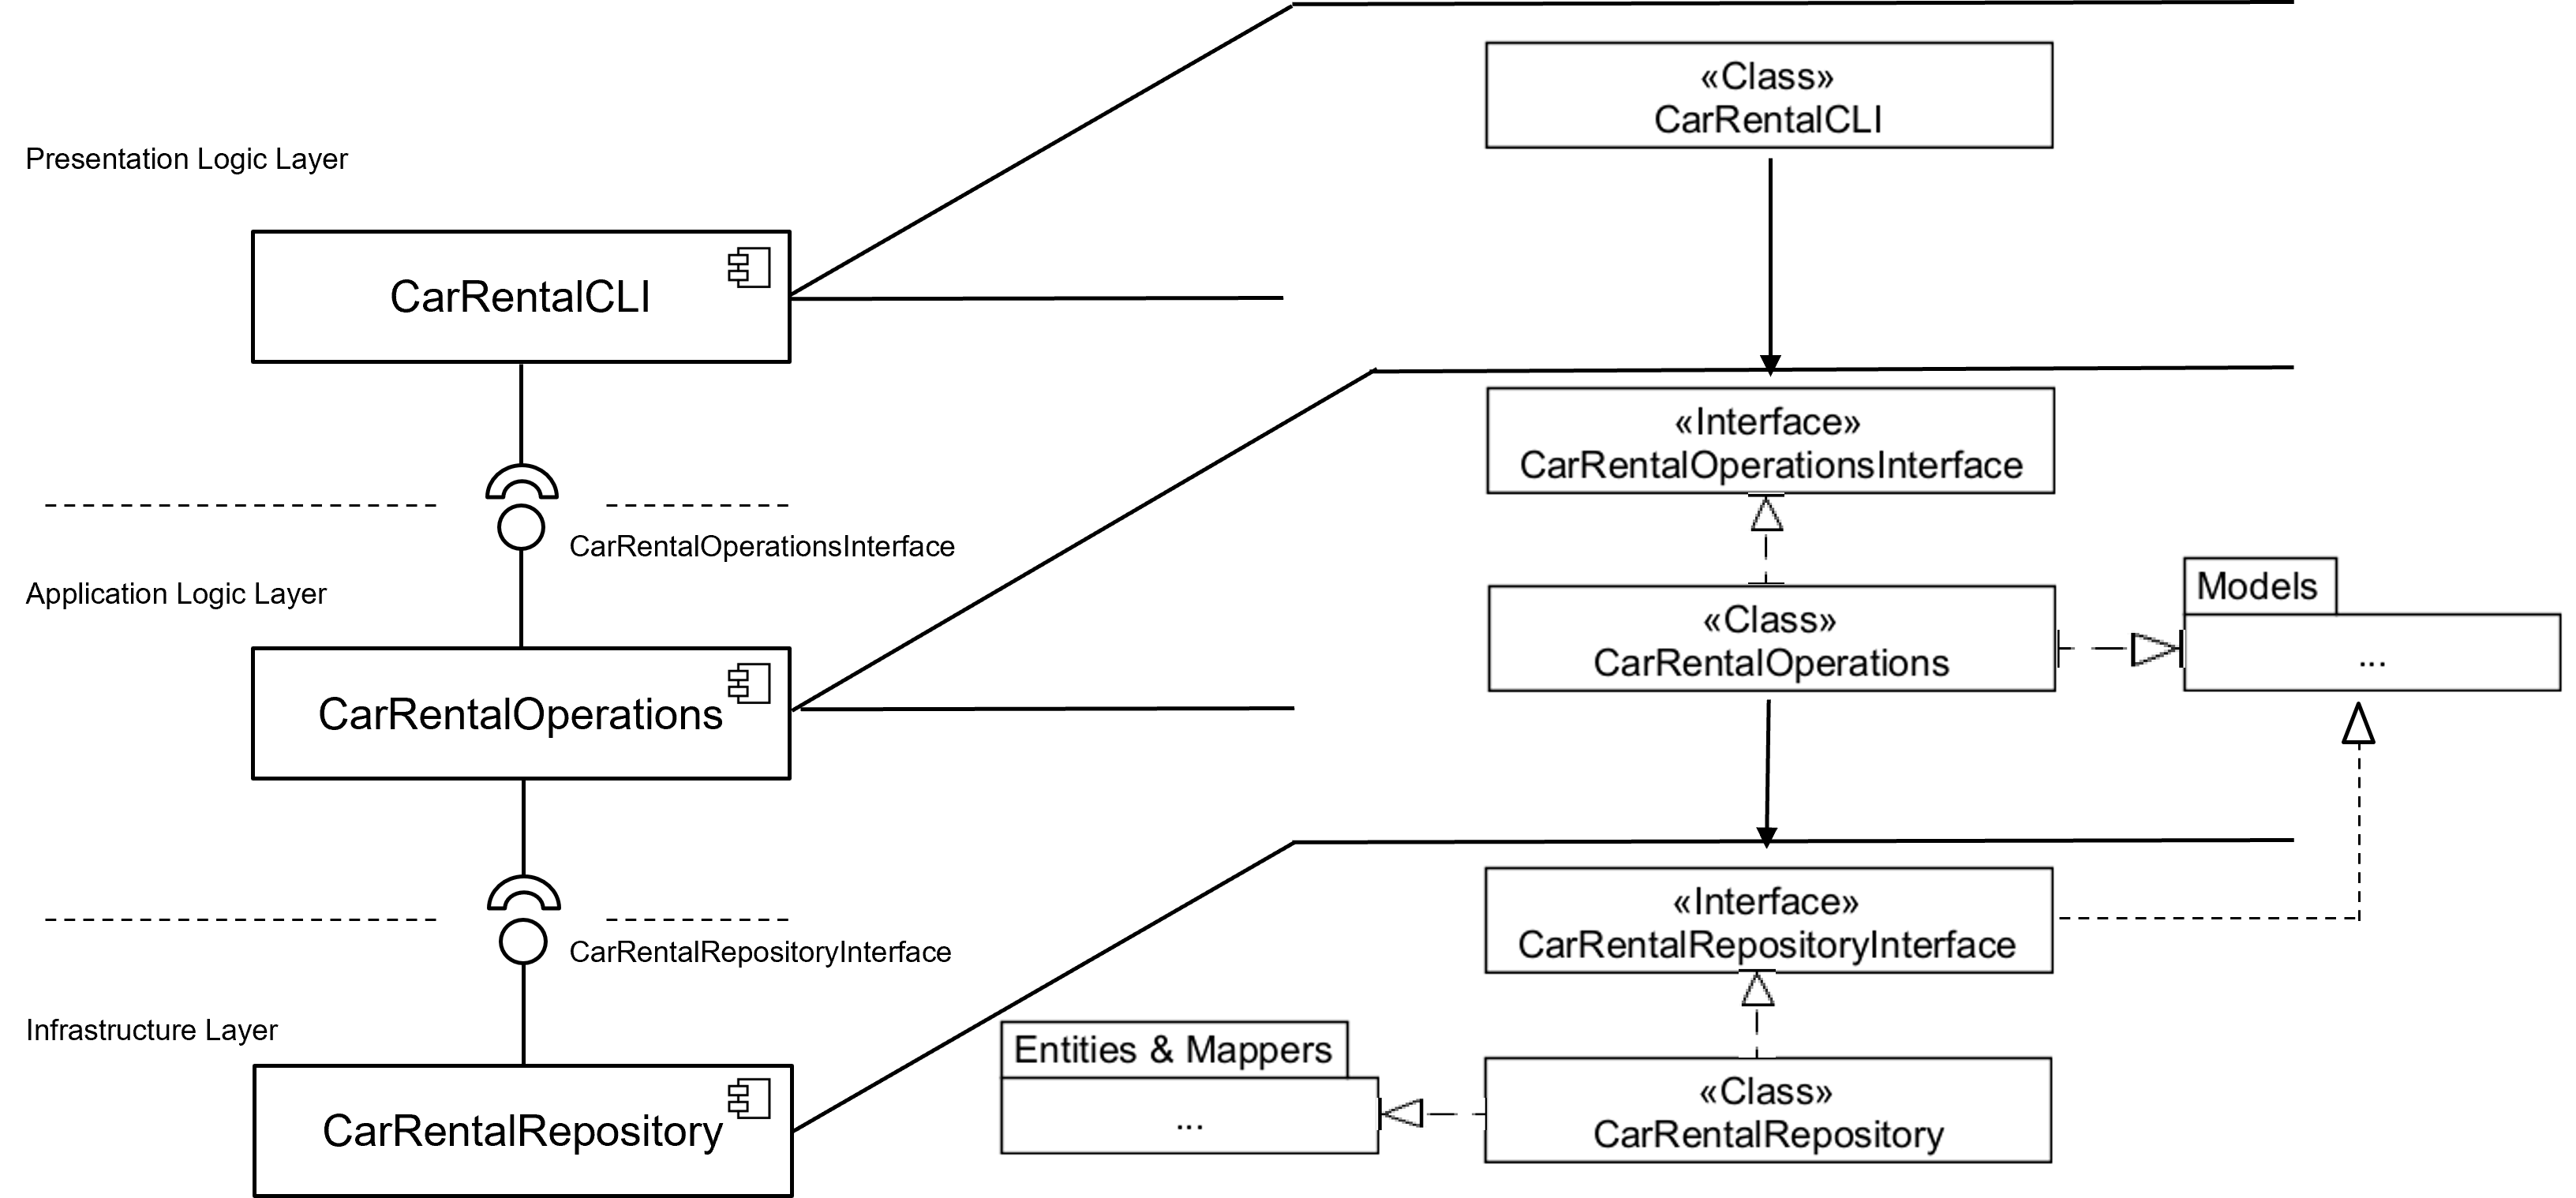
\includegraphics[width=0.8\textwidth]{figures/goLang/carRental/carRentalCLI/carRentalCLI_MicroArchitecture.png}
      \caption{Micro Architecture of the CarRentalCLI}
      \label{fig:car_rental_cli_micro_architecture}
\end{figure}

\subsubsection*{Start the Go Program CarRentalCLI}
The program is started by running \texttt{go run . --- rent} in the \texttt{./CarRentalCLI} directory.

The program asks for the ID of the customer and the ID of the car.
After entering the IDs, the program asks for the start and end date of the rental by asking for the day, month and year.
If the data is entered correctly and the rental is successful, the program prints a success message and exits.
Otherwise, the program asks for the remaining data and prints an error message, the exit status and exits.

The successful execution of the program is displayed in \autoref{fig:car_rental_cli_successful_rental_max}.

\begin{figure}
      \centering
      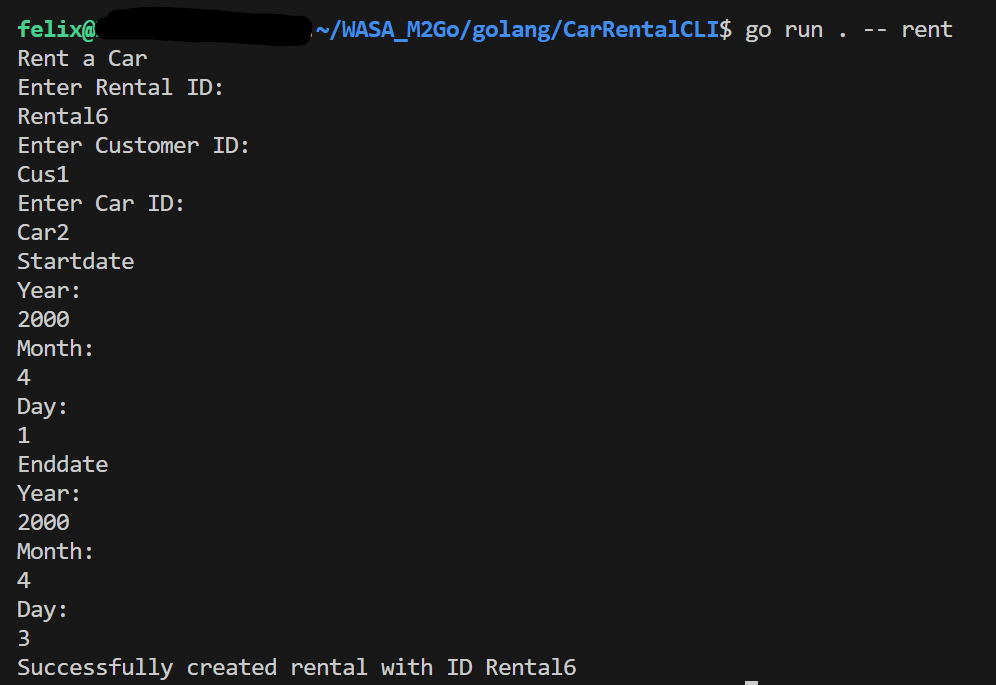
\includegraphics[width=0.8\textwidth]{figures/goLang/carRental/carRentalCLI/carRentalCli_SuccessfulRentalMax.png}
      \caption{Successful Rental of a Car for Max}
      \label{fig:car_rental_cli_successful_rental_max}
\end{figure}

\subsection{Excercise AddRegisterAsCustomer}
\label{sec:exercise_add_register_as_customer}
This task adds the functionality to register as a customer.

To fulfill this task, the following steps are required:
First, a CLI command is added to the presentation layer which calls the basic functions to register a new customer.
After that, an entity mapper is added to the infrastructure layer.
Then, the operation is implemented including validations.
The last step is to test the functionality by registering Alice as a customer.

This is a hands-on task, which requires adding code to the existing application.

\subsubsection*{Add CLI Command}
The CLI commands are placed in the \texttt{CarRentalCLI.go} file.
The \texttt{NewCarRentalCLI} function takes \texttt{operations.CarRentalOperations} as input and returns a \texttt{CarRentalCLI} object that can be executed.
This function also specifies the commands that can be executed by the CLI.
The array \texttt{Commands} contains these commands consisting of the name, the usage, and the according action.

To add the command for registering a new customer, the array \texttt{Commands} is extended by the command \texttt{register} with the usage \texttt{Register as Customer}.
The action defines a function taking a CLI-context object as input and returning an error.
This function calls the according function that executes the code executing the actual task.

The code for the new CLI command \texttt{register} is shown in \autoref{lst:car_rental_cli_command_register}.
The new customer is created in \autoref{lst:car_rental_cli_create_customer_persistence_entity}.

\begin{lstlisting}[
      float=h,
      style=kit-cm,
      caption={Code for the CLI Command "register"},
      label={lst:car_rental_cli_command_register},
      language=Golang
]
...
// array and function definition
... // other commands
{
      Name:  "register",
      Usage: "Register as Customer",
      Action: func(cCtx *cli.Context) error {
            return RegisterAsCustomerAction(operations)
      },
},
... // other commands
\end{lstlisting}

\begin{lstlisting}[
      float=h,
      style=kit-cm,
      caption={Creating a Customer Persistence Entity},
      label={lst:car_rental_cli_create_customer_persistence_entity},
      language=Golang
]
// file: CarRentalRepository.go
...
func (repository CarRentalRepository) CreateCustomer(customer model.Customer) error {
	var newCustomer = YAMLMapper.ConvertCustomerToCustomerPersistenceEntity(customer)

	repository.Customers = append(repository.Customers, newCustomer)
	repository.SaveData()
	return nil
}
...
\end{lstlisting}

\subsubsection*{Add Entity Mapper}
What is the necessity for a mapper?
The general task of a mapper is to enable communication between the application and the database.
In this case, the database is a yaml file.
Therefore the mapper can read and write to the yaml files and convert the data to the corresponding entities and vice versa.

Also, mappers are important in terms of decoupling.
They give the possibility to switch the infrastructure layer by adjusting the mappers only.

In the use case of registering a new customer, the mapper is called while creating a new customer.
This mapper is located in the \texttt{./CustomerMapper.go} file, containing two functions.
The first function \texttt{ConvertCustomerToCustomerPersistenceEntity} takes a customer object as an argument and returns a customer persistence entity containing the same values.
This entity is then written to the yaml file.
By writing the entity into the yaml file, the customer is registered and can be used in the application.

The second function \texttt{ConvertCustomerPersistenceEntityToCustomer} takes a customer persistence entity as an argument and returns a customer object containing the same values.
It acts just like the function above but in the opposite direction.

This task is about implementing the \texttt{ConvertCustomerToCustomerPersistenceEntity} function.
The code for this function is shown in \autoref{lst:car_rental_cli_mapper_customer_to_customer_persistence_entity}.

\begin{lstlisting}[
      float=h,
      style=kit-cm,
      language=Golang,
      caption={Code for the ConvertCustomerToCustomerPersistenceEntity Function},
      label={lst:car_rental_cli_mapper_customer_to_customer_persistence_entity},
]
// CustomerMapper.go
// author = Felix Weik

func ConvertCustomerToCustomerPersistenceEntity(customer model.Customer) entities.CustomerPersistenceEntity {
return entities.CustomerPersistenceEntity{
      ID:   customer.ID,
      Name: customer.Name,
}
}
\end{lstlisting}

\subsubsection*{Implement Operation}
The registering process is implemented in separate files across the different layers.

The CLI command "register" calls the \texttt{RegisterAsCustomerAction} function starting from the \texttt{CarRentalCLI.go} file.
This function is located in the \texttt{CliActions.go} file.
It prints a message to the CLI and collects the customerID and the customerName attributes via other functions from the CLI package.

After that, it calls the \texttt{RegisterAsCustomer} function that takes both collected \hfill \linebreak values as input.
This function is located in the operations package in the \hfill \linebreak \texttt{RegisterAsCustomerOperation.go} file.
It validates the input by checking if the customer exists.
If the input is valid, it calls the \texttt{NewCustomer} and \texttt{CreateCustomer} functions, which are located in the models package.
These functions will write to the YAML file, storing the new customer.

If an error occurs or the validations fail, the process will abort.
If the process succeeds, a success message containing the newly created customer ID is printed to the CLI.

\subsubsection*{Register Alice as Customer}
After running the CLI command to register a new customer, the program asks for the ID of the customer.
In this case, Alice receives the ID \texttt{Cus5}.
After entering the ID, the program asks for the name of the customer, in this case Alice.
The program exits with a success message and the exit status as shown in \autoref{fig:car_rental_cli_register_alice}.

To register a new rental, the program starts with \texttt{go run . --- rent}.
The program asks for the ID of the rental, here it is \texttt{Rental7}.
The customer ID for Alice is \texttt{Cus5}.
After that, the start and end date is entered.
The program exits with a success message and the exit status as shown in \autoref{fig:car_rental_cli_rental_alice_successful}.

\begin{figure}
      \centering
      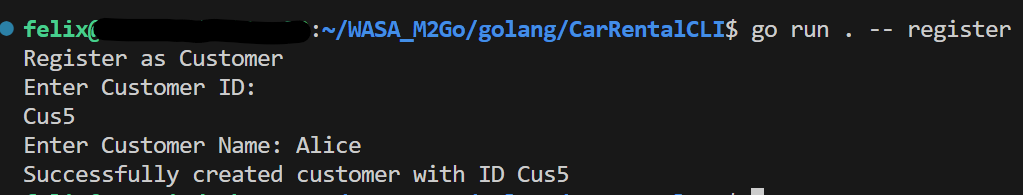
\includegraphics[width=0.8\textwidth]{figures/goLang/carRental/carRentalCLI/carRentalCLI_RegisterAlice.png}
      \caption{Register Alice as a Customer}
      \label{fig:car_rental_cli_register_alice}
\end{figure}
\begin{figure}
      \centering
      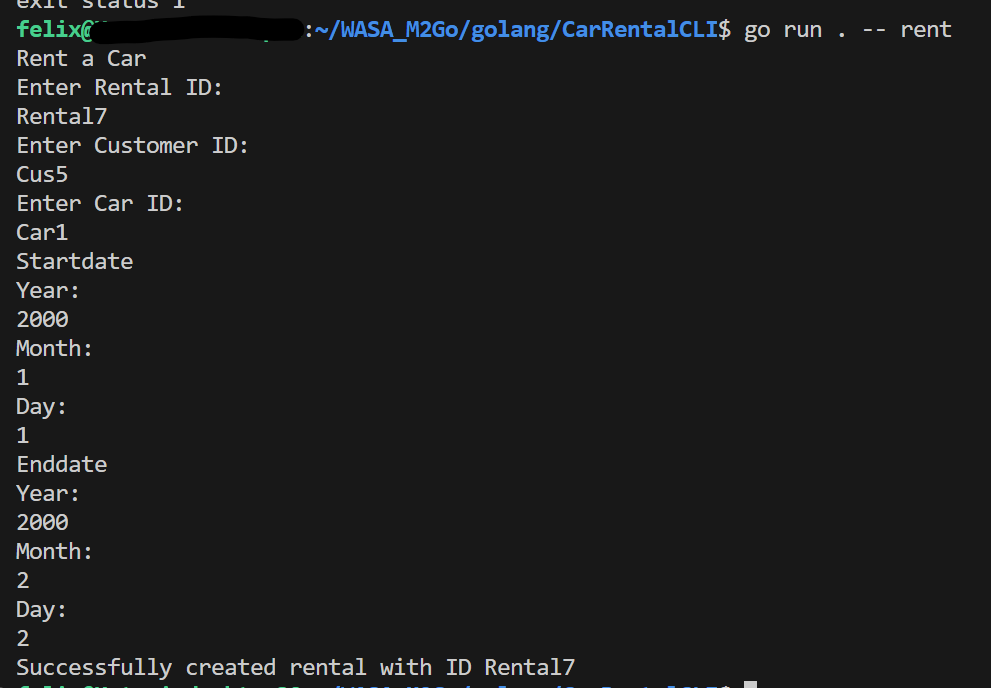
\includegraphics[width=0.8\textwidth]{figures/goLang/carRental/carRentalCLI/carRentalCLI_SuccessfulRentalAlice.png}
      \caption{Successful Rental of a Car for Alice}
      \label{fig:car_rental_cli_rental_alice_successful}
\end{figure}
